% questions.tex —— 1958 年·不明卷（与云南卷部分同源） · 题目内容片段（无答案）
% 由 tools/generate_projects.py 依来源总账自 1958/1958_不明卷_数学真题_试题.md 生成，勿手改（改源 MD 后重跑）


\begin{question}
\gkti{1}若 $\tan\alpha=\dfrac12$，$\tan\beta=\dfrac13$，并且 $\alpha$ 与 $\beta$ 均为锐角。求证：$\alpha+\beta=45^\circ$。

\end{question}
\begin{question}
\gkti{2}问 $k$ 取何值时，二次方程 $(2k-1)x^2+(k+1)x+k-4=0$ 才有等根。

\end{question}
\begin{question}
\gkti{3}求 $(1+x)+(1+x)^2+\cdots+(1+x)^{10}$ 式中 $x^8$ 项的系数，（不必求出其它各项系数）。

\Needspace{0.4\textheight}
\end{question}
\begin{question}
\gkti{4}设一四面体被一平面所截，若截面为一平行四边形，则此截面平行于四面体的两条棱。
\nopagebreak[4]
\begin{center}% 1958 年不明卷（可能是某省与云南试题混合）第 4 题：四面体 ABCD（A 顶部、D 左、B 右、C 底部）被一平面所截，截口 HEFG 为平行四边形（H 在 AD 上、E 在 AC 上、F 在 CB 上、G 在 DB 上）；DB 为背面棱，虚线；截面靠背面的两边 FG、GH 亦随之绘为虚线（按源卷布局，坐标手算）
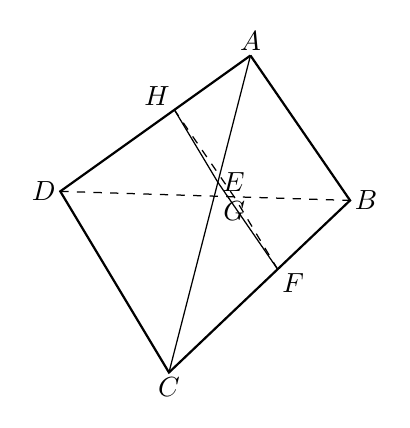
\begin{tikzpicture}[scale=1.15, line width=0.45pt,
  every node/.style={inner sep=1.5pt}]
  \coordinate (A) at (0.5,2.0);
  \coordinate (D) at (-1.6,0.5);
  \coordinate (B) at (1.6,0.4);
  \coordinate (C) at (-0.4,-1.5);
  \coordinate (H) at (-0.34,1.4);
  \coordinate (E) at (0.14,0.6);
  \coordinate (G) at (0.32,0.44);
  \coordinate (F) at (0.8,-0.36);
  \draw[line width=0.8pt] (A) -- (D) -- (C) -- (B) -- (A);
  \draw (A) -- (C);
  \draw[dashed] (D) -- (B);
  \draw (H) -- (E) -- (F);
  \draw[dashed] (F) -- (G) -- (H);
  \node[anchor=south] at (A) {$A$};
  \node[anchor=east] at (D) {$D$};
  \node[anchor=west] at (B) {$B$};
  \node[anchor=north] at (C) {$C$};
  \node[anchor=south east] at (H) {$H$};
  \node[anchor=west] at (E) {$E$};
  \node[anchor=north] at (G) {$G$};
  \node[anchor=north west] at (F) {$F$};
\end{tikzpicture}
\end{center}
\nopagebreak[4]
\end{question}
\begin{question}
\gkti{5}设三角形 $ABC$ 中，角 $A$ 的外角平分线与 $BC$ 边之延长线交于 $D$，与外接圆周交于 $E$，则：$AB\cdot AC=AE\cdot AD$。

\end{question}
\begin{question}
\gkti{6}设有互相外切的二圆，半径各为 $a$ 与 $b$（$a>b$），作此二圆的两条外公切线，设其夹角为 $A$，证明：

\nopagebreak[4]
\[
\sin A=\frac{4(a-b)\sqrt{ab}}{(a+b)^2}
\]

\end{question}
\begin{question}
\gkti{7}在三角形 $ABC$ 中，$r$、$R$ 分别为其内切圆与外接圆的半径。求证：

\nopagebreak[4]
\[
r=4R\sin\frac A2\sin\frac B2\sin\frac C2
\]

\end{question}
\begin{question}
\gkti{8}解方程：

\nopagebreak[4]
\[
\sqrt[3]{4a^3+x}+\sqrt[3]{4a^3-x}=2a
\]

\end{question}